% Sato-Tate: histogram of a_p/(2 sqrt p) for y^2=x^3-x+1, p<10^6 (generated by a script).
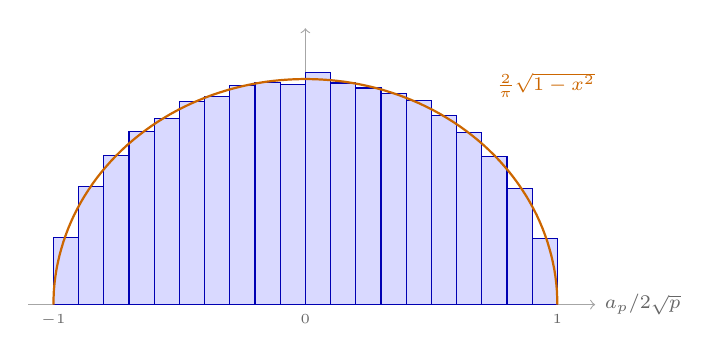
\begin{tikzpicture}[x=1cm,y=1cm]
\draw[black!35,->] (-3.52,0)--(3.68,0) node[right,font=\scriptsize,black!60]{$a_p/2\sqrt p$};
\draw[black!35,->] (0,0)--(0,3.51);
\draw[blue!70!black,fill=blue!15] (-3.200,0) rectangle (-2.880,0.847);
\draw[blue!70!black,fill=blue!15] (-2.880,0) rectangle (-2.560,1.503);
\draw[blue!70!black,fill=blue!15] (-2.560,0) rectangle (-2.240,1.899);
\draw[blue!70!black,fill=blue!15] (-2.240,0) rectangle (-1.920,2.199);
\draw[blue!70!black,fill=blue!15] (-1.920,0) rectangle (-1.600,2.366);
\draw[blue!70!black,fill=blue!15] (-1.600,0) rectangle (-1.280,2.580);
\draw[blue!70!black,fill=blue!15] (-1.280,0) rectangle (-0.960,2.641);
\draw[blue!70!black,fill=blue!15] (-0.960,0) rectangle (-0.640,2.781);
\draw[blue!70!black,fill=blue!15] (-0.640,0) rectangle (-0.320,2.823);
\draw[blue!70!black,fill=blue!15] (-0.320,0) rectangle (0.000,2.790);
\draw[blue!70!black,fill=blue!15] (0.000,0) rectangle (0.320,2.951);
\draw[blue!70!black,fill=blue!15] (0.320,0) rectangle (0.640,2.815);
\draw[blue!70!black,fill=blue!15] (0.640,0) rectangle (0.960,2.751);
\draw[blue!70!black,fill=blue!15] (0.960,0) rectangle (1.280,2.683);
\draw[blue!70!black,fill=blue!15] (1.280,0) rectangle (1.600,2.594);
\draw[blue!70!black,fill=blue!15] (1.600,0) rectangle (1.920,2.407);
\draw[blue!70!black,fill=blue!15] (1.920,0) rectangle (2.240,2.185);
\draw[blue!70!black,fill=blue!15] (2.240,0) rectangle (2.560,1.882);
\draw[blue!70!black,fill=blue!15] (2.560,0) rectangle (2.880,1.469);
\draw[blue!70!black,fill=blue!15] (2.880,0) rectangle (3.200,0.835);
\draw[orange!80!black,thick] (-3.200,0.000) -- (-3.198,0.090) -- (-3.194,0.180) -- (-3.186,0.270) -- (-3.175,0.359) -- (-3.161,0.448) -- (-3.143,0.537) -- (-3.123,0.625) -- (-3.099,0.712) -- (-3.073,0.799) -- (-3.043,0.885) -- (-3.011,0.970) -- (-2.975,1.055) -- (-2.937,1.138) -- (-2.895,1.220) -- (-2.851,1.301) -- (-2.804,1.380) -- (-2.754,1.458) -- (-2.702,1.535) -- (-2.647,1.610) -- (-2.589,1.684) -- (-2.528,1.756) -- (-2.466,1.826) -- (-2.400,1.895) -- (-2.333,1.961) -- (-2.263,2.026) -- (-2.191,2.088) -- (-2.116,2.149) -- (-2.040,2.207) -- (-1.961,2.264) -- (-1.881,2.318) -- (-1.799,2.369) -- (-1.715,2.419) -- (-1.629,2.466) -- (-1.542,2.510) -- (-1.453,2.553) -- (-1.362,2.592) -- (-1.271,2.629) -- (-1.178,2.664) -- (-1.084,2.695) -- (-0.989,2.725) -- (-0.893,2.751) -- (-0.796,2.775) -- (-0.698,2.796) -- (-0.600,2.814) -- (-0.501,2.830) -- (-0.401,2.842) -- (-0.301,2.852) -- (-0.201,2.859) -- (-0.101,2.863) -- (0.000,2.865) -- (0.101,2.863) -- (0.201,2.859) -- (0.301,2.852) -- (0.401,2.842) -- (0.501,2.830) -- (0.600,2.814) -- (0.698,2.796) -- (0.796,2.775) -- (0.893,2.751) -- (0.989,2.725) -- (1.084,2.695) -- (1.178,2.664) -- (1.271,2.629) -- (1.362,2.592) -- (1.453,2.553) -- (1.542,2.510) -- (1.629,2.466) -- (1.715,2.419) -- (1.799,2.369) -- (1.881,2.318) -- (1.961,2.264) -- (2.040,2.207) -- (2.116,2.149) -- (2.191,2.088) -- (2.263,2.026) -- (2.333,1.961) -- (2.400,1.895) -- (2.466,1.826) -- (2.528,1.756) -- (2.589,1.684) -- (2.647,1.610) -- (2.702,1.535) -- (2.754,1.458) -- (2.804,1.380) -- (2.851,1.301) -- (2.895,1.220) -- (2.937,1.138) -- (2.975,1.055) -- (3.011,0.970) -- (3.043,0.885) -- (3.073,0.799) -- (3.099,0.712) -- (3.123,0.625) -- (3.143,0.537) -- (3.161,0.448) -- (3.175,0.359) -- (3.186,0.270) -- (3.194,0.180) -- (3.198,0.090) -- (3.200,0.000);
\node[below,font=\tiny,black!60] at (-3.2,0) {$-1$};
\node[below,font=\tiny,black!60] at (0.0,0) {$0$};
\node[below,font=\tiny,black!60] at (3.2,0) {$1$};
\node[font=\scriptsize,orange!80!black,anchor=west] at (2.30,2.79) {$\frac2\pi\sqrt{1-x^2}$};
\end{tikzpicture}
